\documentclass[12pt]{jarticle}
\usepackage[dvipdfmx]{graphicx}
\usepackage{url}
\usepackage{listings,jlisting}
\usepackage{ascmac}
\usepackage{amsmath,amssymb}

%ここからソースコードの表示に関する設定
\lstset{
  basicstyle={\ttfamily},
  identifierstyle={\small},
  commentstyle={\smallitshape},
  keywordstyle={\small\bfseries},
  ndkeywordstyle={\small},
  stringstyle={\small\ttfamily},
  frame={tb},
  breaklines=true,
  columns=[l]{fullflexible},
  numbers=left,
  xrightmargin=0zw,
  xleftmargin=3zw,
  numberstyle={\scriptsize},
  stepnumber=1,
  numbersep=1zw,
  lineskip=-0.5ex
}
%ここまでソースコードの表示に関する設定

\title{知能プログラミング演習II 課題5}
\author{グループ8\\
  29114003 青山周平\\
}
\date{2020年1月6日}

\begin{document}
\maketitle

\paragraph{提出物} work6
\paragraph{グループ} グループ8
\paragraph{メンバー}
\begin{tabular}{|c|c|c|}
  \hline
  学生番号&氏名&貢献度比率\\
  \hline\hline
  29114003&青山周平&20\\
  \hline
  29114060&後藤拓也&20\\
  \hline
  29114116&増田大輝&20\\
  \hline
  29114142&湯浅範子&20\\
  \hline
  29119016&小中祐希&20\\
  \hline
\end{tabular}

\section{課題の説明}
\begin{description}
\item[必須課題6-1] 課題5にやり残した発展課題があれば参考にして拡張しても良いし,全く新しい独自仕様を考案しても構わない.自由に拡張するか,あるいはもし残っていた問題点があれば完成度を高めよ.
\end{description}

\section{必須課題6-1}
\begin{screen}
課題5にやり残した発展課題があれば参考にして拡張しても良いし,全く新しい独自仕様を考案しても構わない.自由に拡張するか,あるいはもし残っていた問題点があれば完成度を高めよ.
\end{screen}
私の担当箇所は,発展課題5-7に対してUnityを用いて実装したプログラムの,GUI改善やプランニングへの機能追加である.

\subsection{手法}
発展課題5-7では,ブロックワールドにおけるプランニングを実現するための過程として,以下のような実装を行った.
\begin{enumerate}
\item 空間やプランに関するオブジェクトの生成.
\item プランニングを行うための,オブジェクトの動作等に関するスクリプトの作成.
\end{enumerate}

これに引き続いて今回は,ブロックワールドにおけるプランニングを実現するために,以下のような方針を立てた.
\begin{enumerate}
\item プランに用いるオブジェクトをより正確に生成できるようにする.
\item プランニングの情報を可視化する.
\end{enumerate}

1.に関して,GUIを画面上に表示することで,オブジェクトを名前や色,形を指定した上で生成できるようにするとともに,オブジェクトの情報を一覧で表示して生成したオブジェクトの管理を視覚的に行えるような仕様とした.

2.に関して,1.で作成する一覧と関連して,選択したオブジェクトの情報が画面左下のステータスバーで確認できるようにした.また,どの物体についての情報が表示されているかを視覚的に確認できるように,選択中のオブジェクトのアウトラインが表示されるような仕様とした.

\subsection{実装}
発展課題5-7で作ったオブジェクトは以下の通りである.
\begin{description}
\item[Main Camera] 主カメラに関するオブジェクト.Room全体をやや見下ろし気味に映す.
\item[Directional Light] オブジェクト全体を照らす照明.
\item[Master] スクリプトをアタッチするための空オブジェクト.
\item[Room] 6個のPlaneオブジェクトを子に持つ,立方体の部屋を構成するオブジェクト.
\item[Cube] 直方体のブロックを生成するプレハブ.
\item[Sphere] 球のブロックを生成するプレハブ.
\item[Torus] 円環体のブロックを生成するプレハブ.
\end{description} 

新しく作った主なオブジェクトは以下の通りである.
\begin{description}
\item[EventSystem] GUIにおいてButtonやInputFieldを機能させるための,フォーカス情報等を掌るオブジェクト.
\item[Canvas] Generator,Preparator,Staterを子オブジェクトに持つ,GUIの大元となるオブジェクト.
\item[Generator] オブジェクトを生成するためのパネル.子オブジェクトにInputFieldName,DropdownColor,DropdownShape,ButtonGenを持つ.
\item[Preparator] 生成したオブジェクトの一覧を管理するパネル.子オブジェクトにScrollView,ButtonRm,ButtonPlanningを持つ.
\item[Stater] オブジェクトの情報等を表示するためのパネル.子オブジェクトにTextStatus,Scrollbarを持つ.
\item[ListObj] PreparatorにおけるScrollViewの要素となるプレハブ.
\end{description} 

C\#スクリプトでは以下のものが実装されている.
\begin{description}
\item[Clicked] クリックされたオブジェクトにフォーカスを当てるスクリプト.Masterにアタッチされる.
\item[Operationg] Clickedでフォーカスされたオブジェクトにキーボード入力を反映するスクリプト.Masterにアタッチされる.
\item[Generator] Generatorオブジェクトで得た情報に合わせて,ブロックを生成するスクリプト.ButtonGenにアタッチされる.
\item[Destroyer] Preparatorオブジェクトで選択されたブロックを削除するためのスクリプト.ButtonRmにアタッチされる.
\item[Manager] ListObjプレハブにアタッチされる,各インスタンスが1対1で対応するブロックを保持するためのスクリプト.
\item[SelectOnList] ListObjプレハブにアタッチされる,インスタンスが自身にアウトラインや削除のフォーカスを当てるためのスクリプト.
\item[Starter] GUIの一部を非表示にし,プランニングを開始するためのスクリプト.ButtonPlanningにアタッチされる.
\item[CollisionGetter] 自身と衝突中のブロックを保持するスクリプト.各ブロックにアタッチされる.
\item[StateGetter] SelectOnListでフォーカスされたブロックと衝突中のブロックをStaterに表示するスクリプト.Masterにアタッチされる.
\end{description}

\subsubsection{プランに用いるオブジェクトをより正確に生成できるようにする.}


\subsubsection{プランニングの情報を可視化する.}

\clearpage

\subsection{実行例}
Block World Planning.exeを起動したところ,下図のような画面が得られる.

\begin{figure}[!hbt]
  	\begin{center}
  		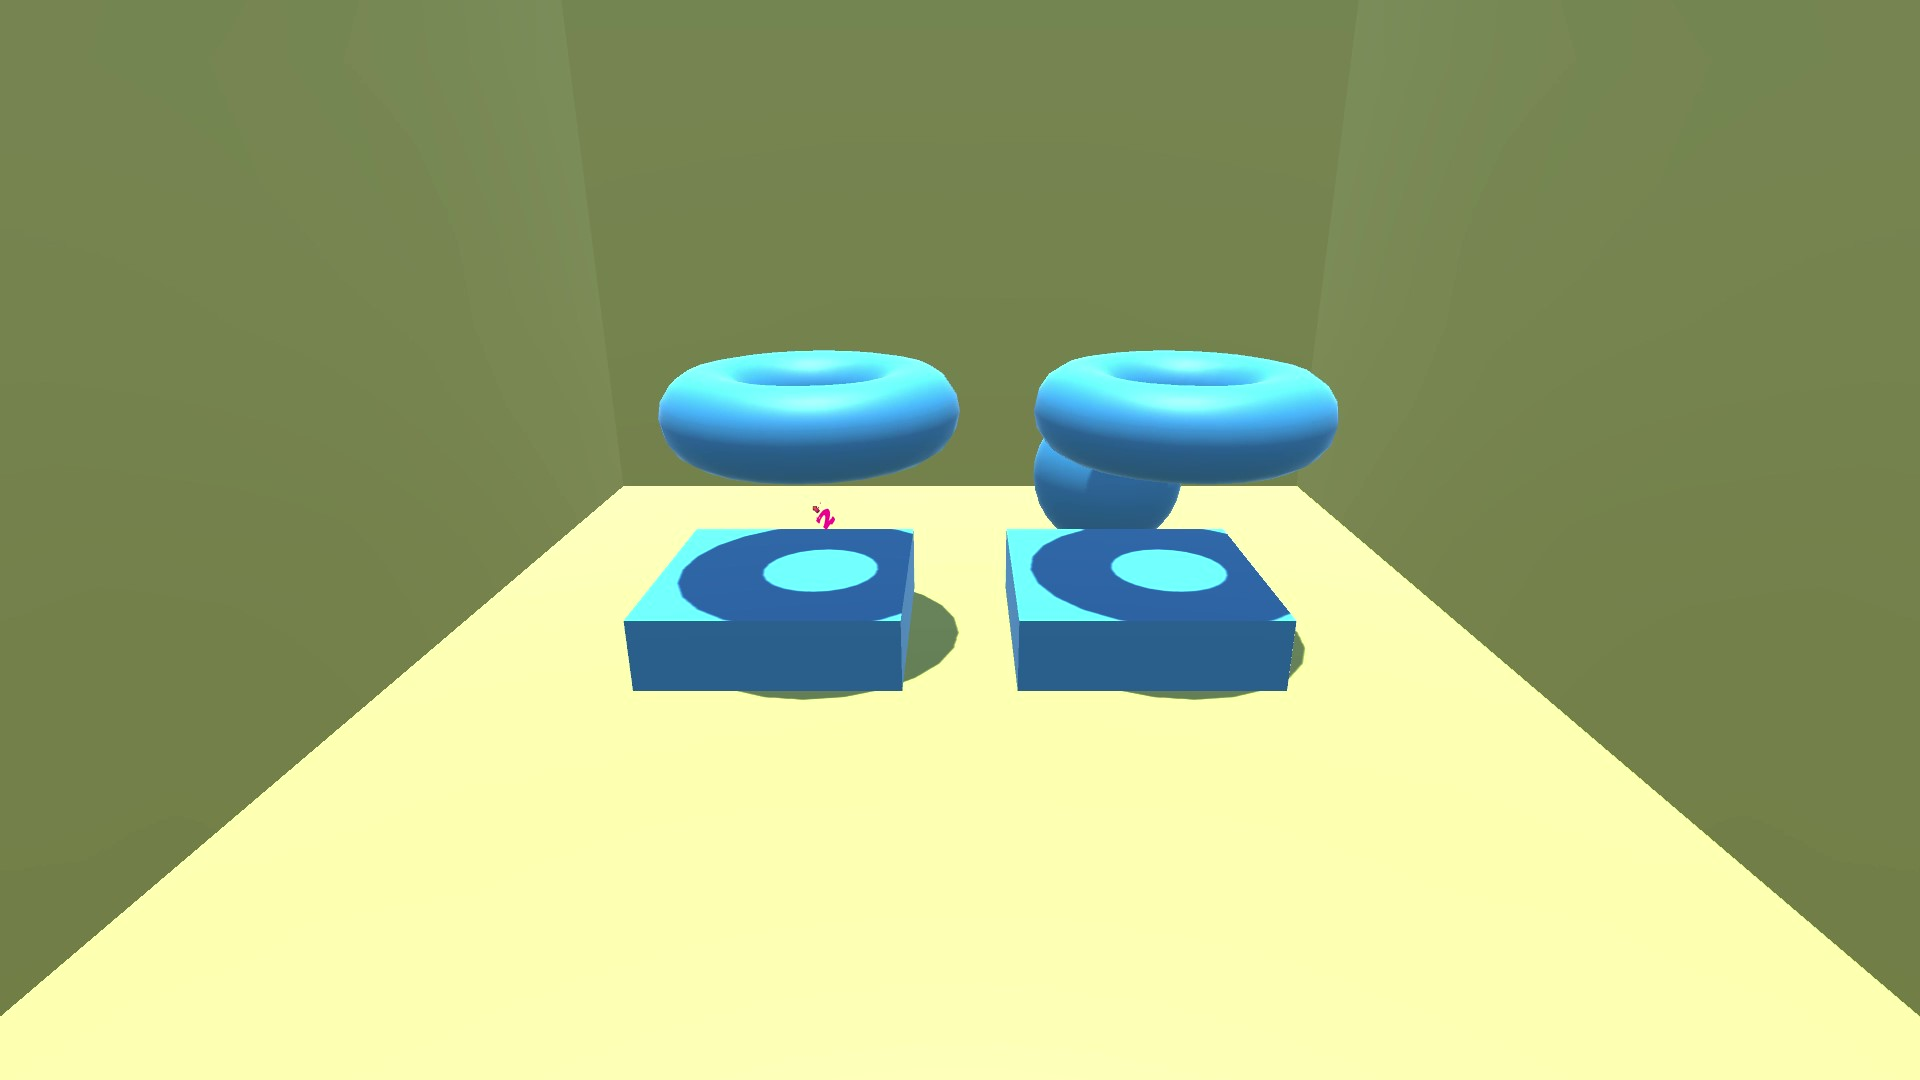
\includegraphics[scale=0.2]{images/bwp3.jpg}
	\end{center}
  	\caption{起動時の画面}
\end{figure}
\clearpage

右クリックでオブジェクトを削除でき,キー``1''で直方体,キー``2''で円環体,キー``3''で球のブロックを生成できる.これによって構成した下図をプランニングの初期状態とする.

\begin{figure}[!hbt]
  	\begin{center}
  		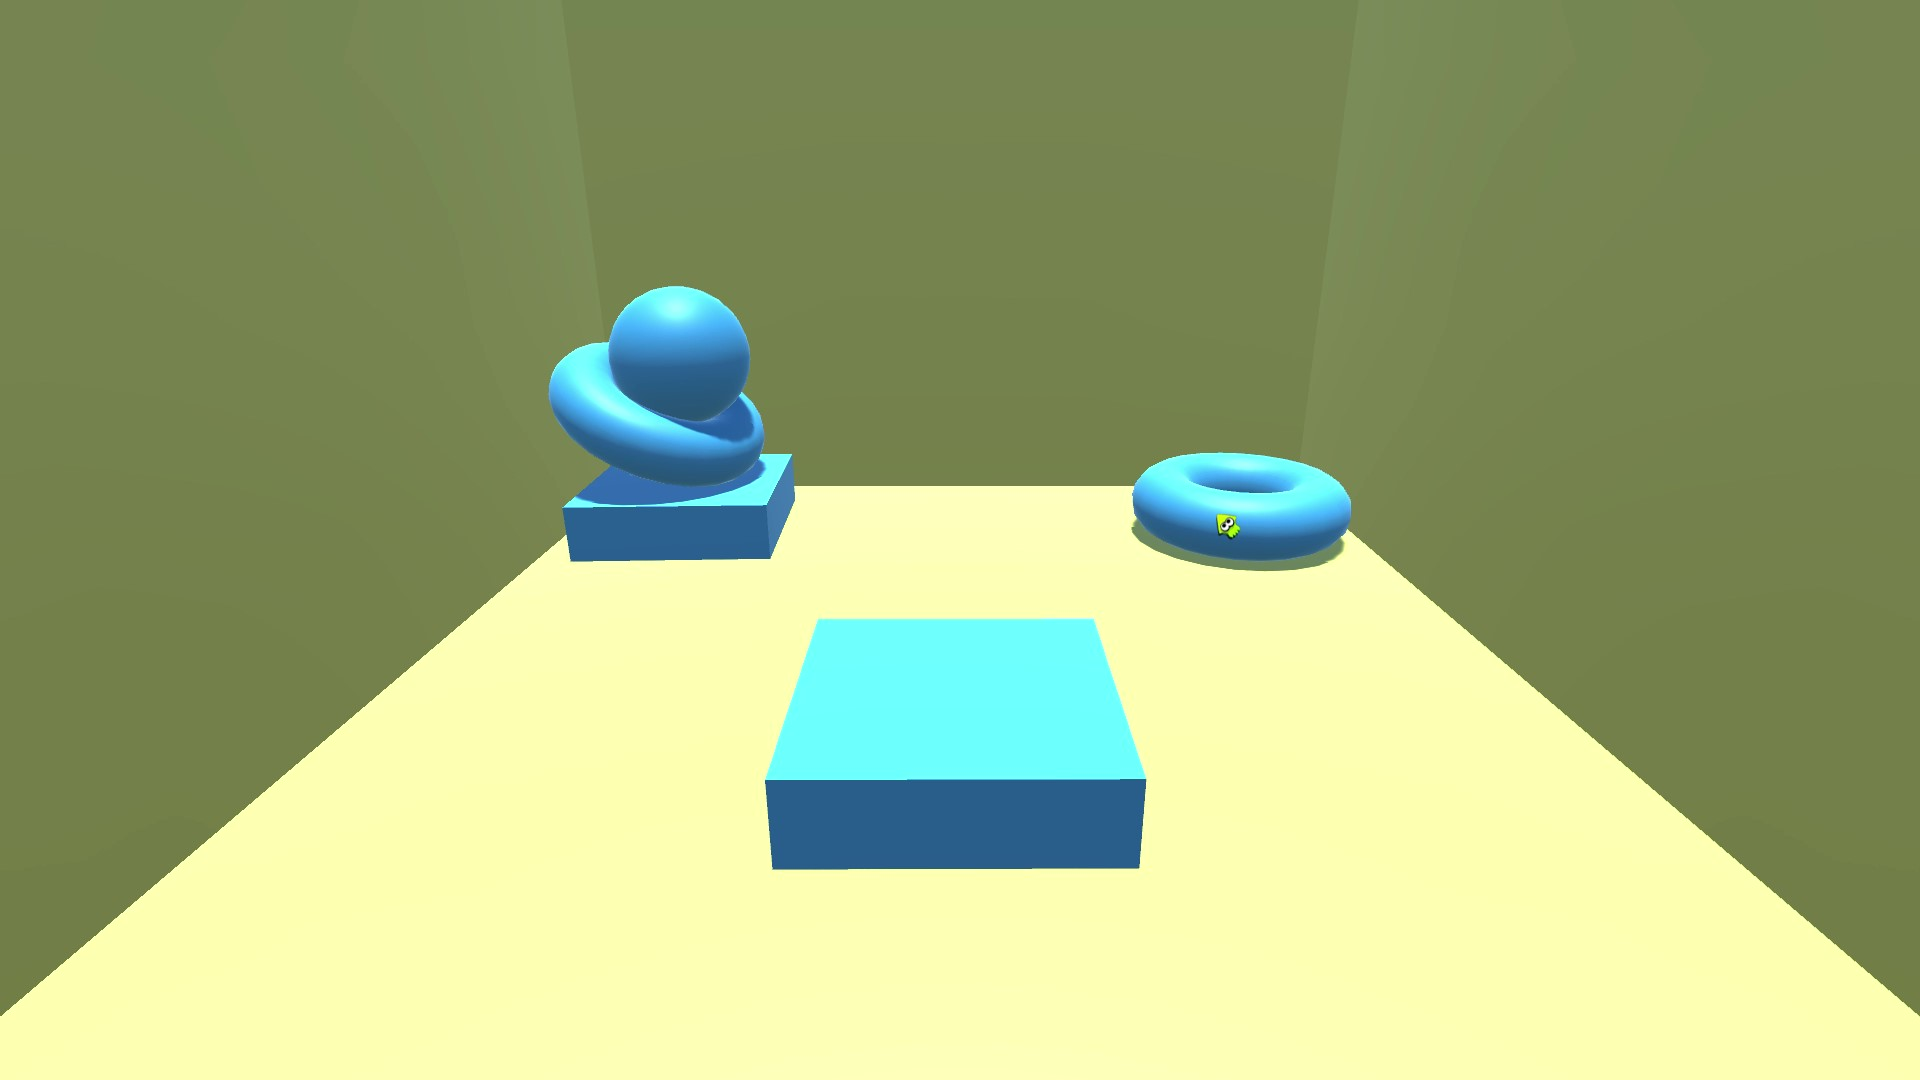
\includegraphics[scale=0.2]{images/bwp4.jpg}
	\end{center}
  	\caption{初期状態}
\end{figure}
\clearpage

左クリックで移動するオブジェクトを選択してから,WASDキーで上下左右,EQキーで昇降の移動が行える.手前の直方体に乗せるために右奥の円環体を持ち上げた様子が下図のとおりである.

\begin{figure}[!hbt]
  	\begin{center}
  		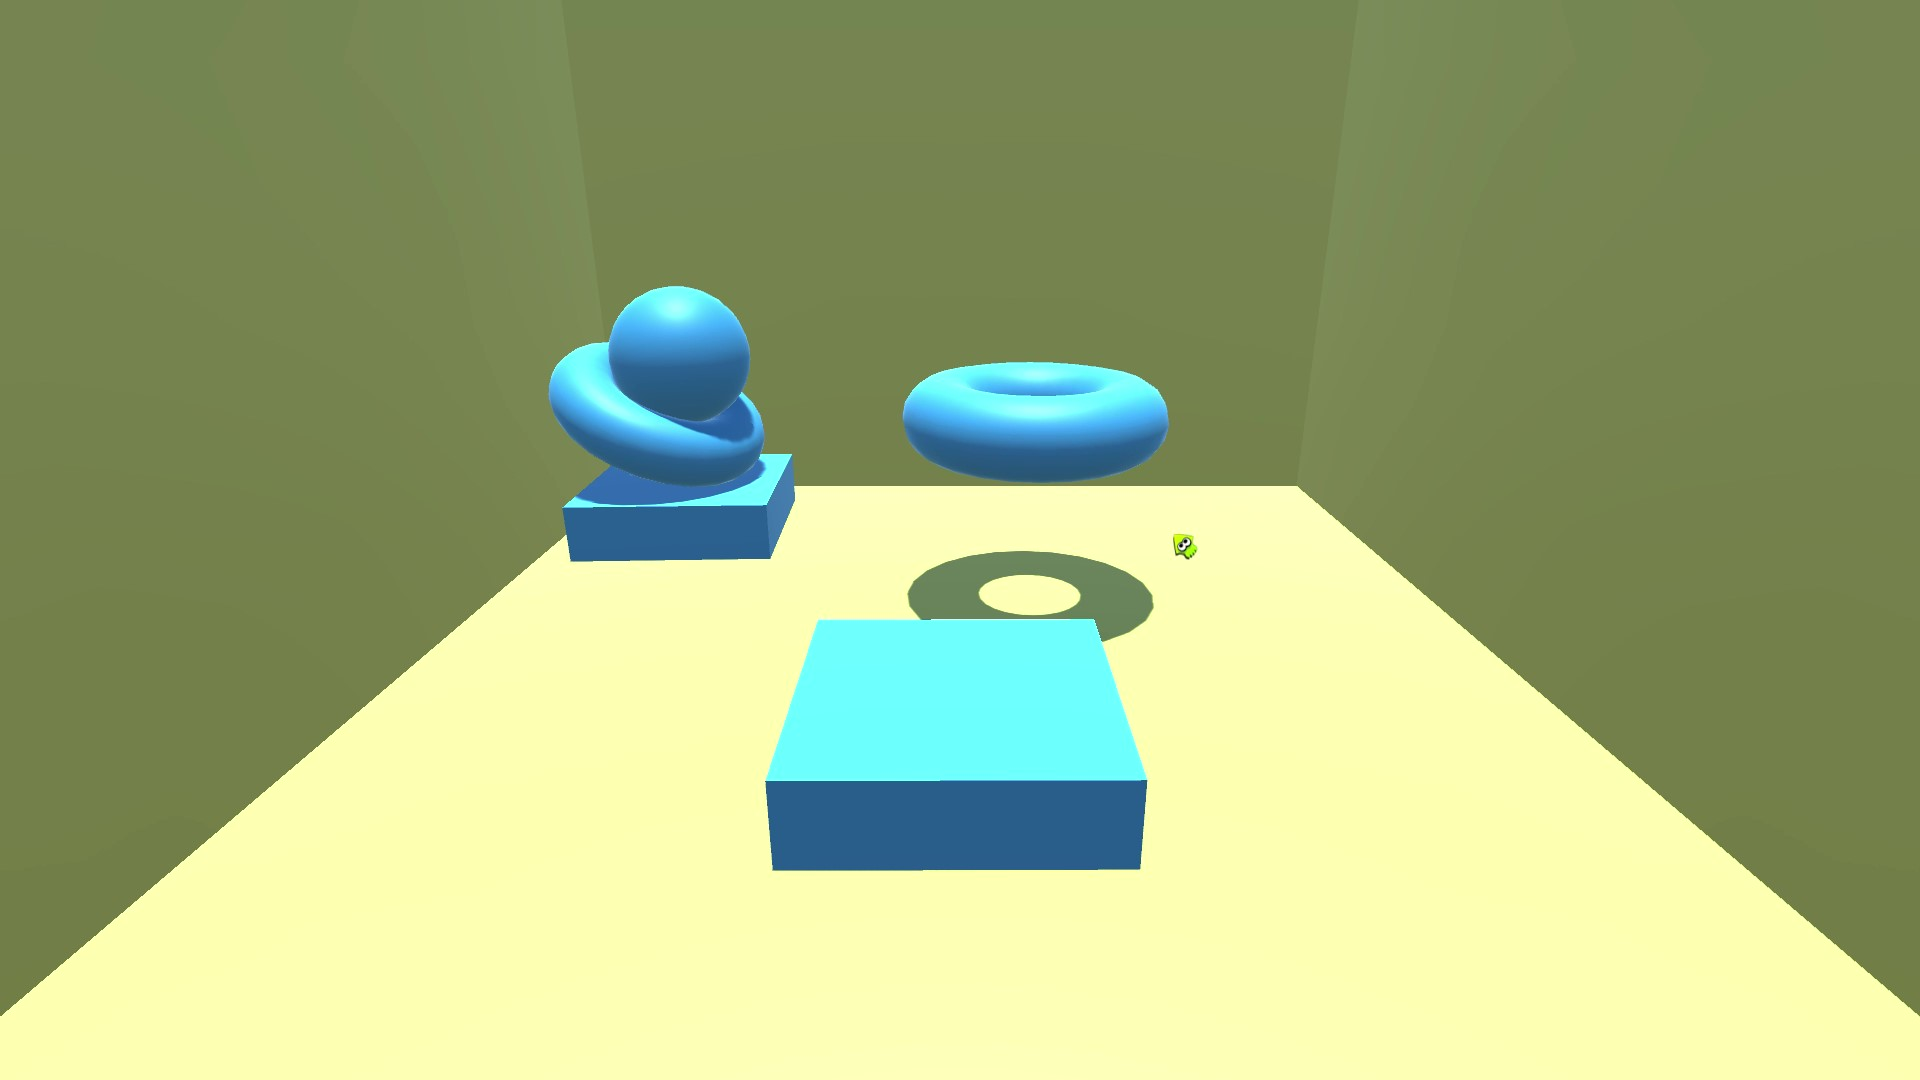
\includegraphics[scale=0.2]{images/bwp5.jpg}
	\end{center}
  	\caption{プランニング開始}
\end{figure}
\clearpage

そうして,物理的な挙動を考慮した上で円環体を直方体の上に乗せた様子が下図のとおりである.

\begin{figure}[!hbt]
  	\begin{center}
  		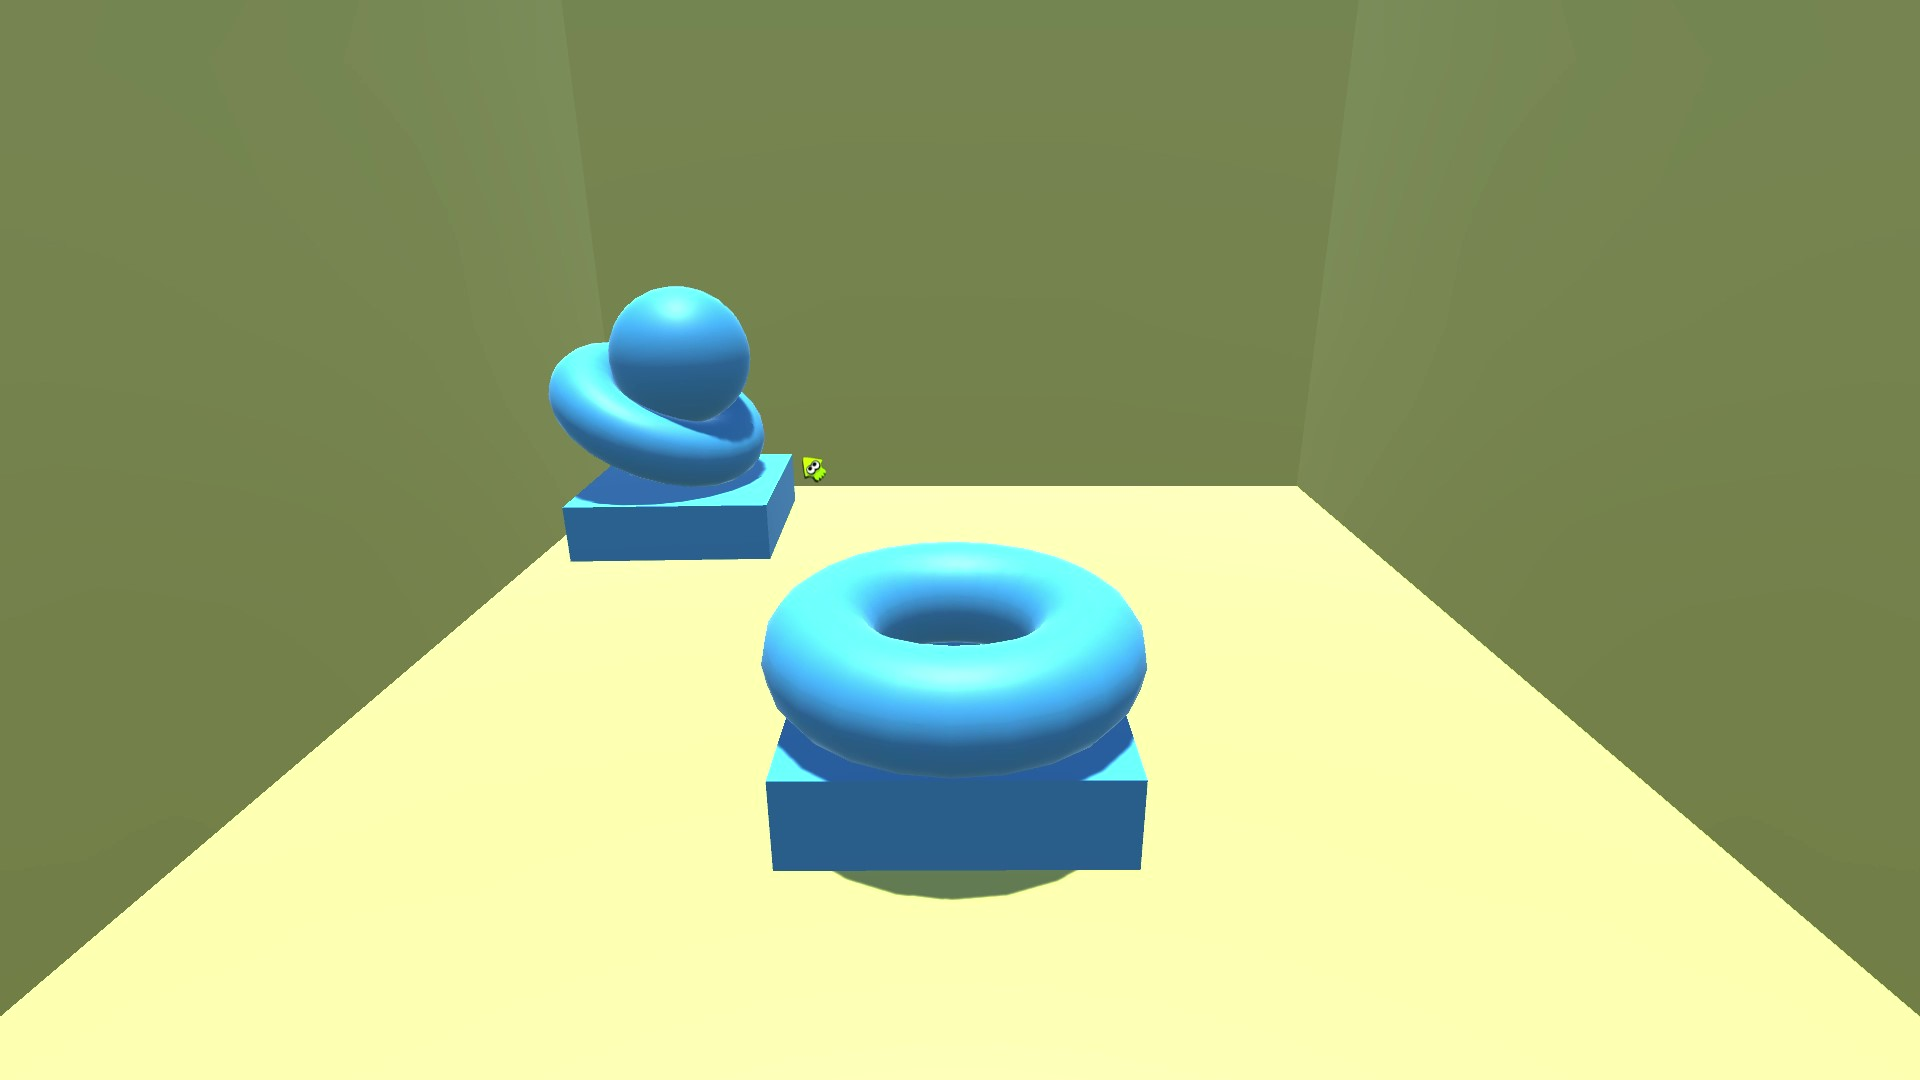
\includegraphics[scale=0.2]{images/bwp6.jpg}
	\end{center}
  	\caption{ステップ1完了}
\end{figure}
\clearpage

物理的な挙動を考慮して完了したプランニングが下図のとおりである.

\begin{figure}[!hbt]
  	\begin{center}
  		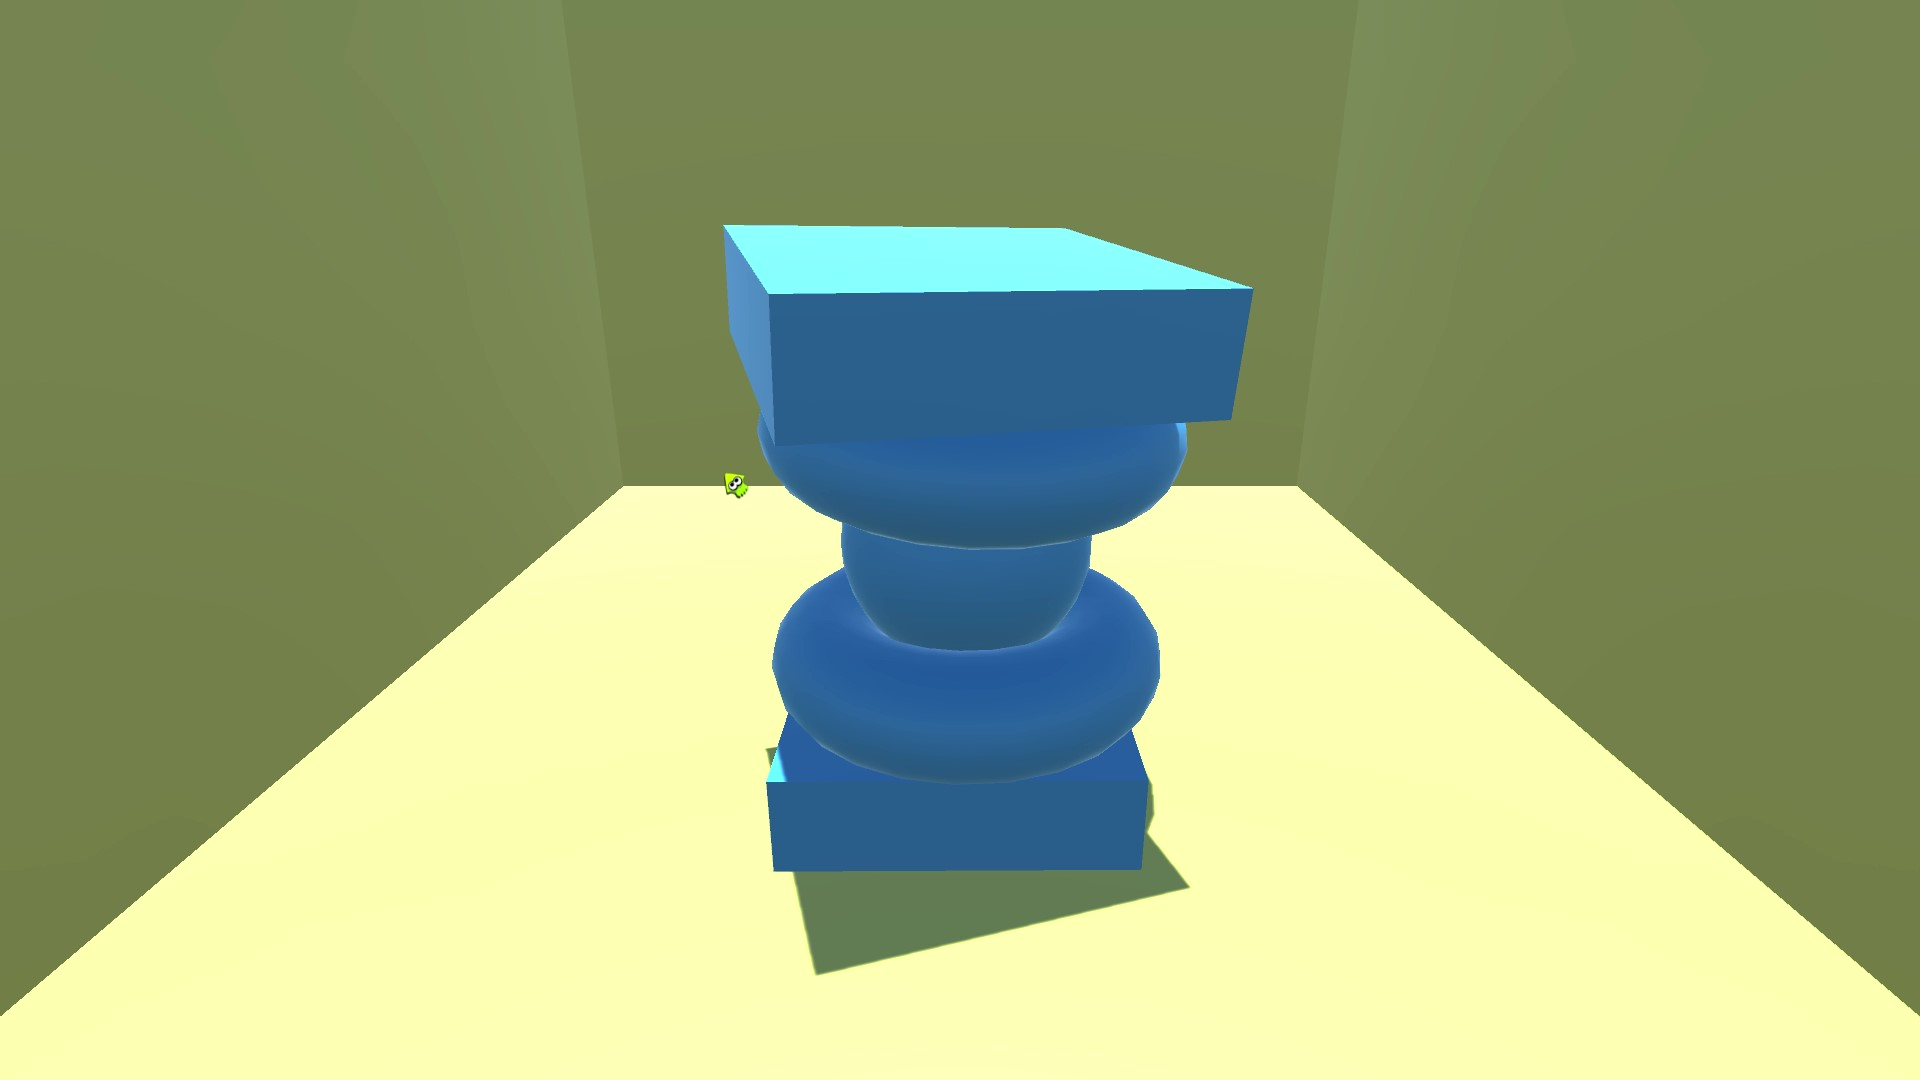
\includegraphics[scale=0.2]{images/bwp7.jpg}
	\end{center}
  	\caption{プランニング完了}
\end{figure}
\clearpage

\subsection{考察}


\section{感想}


% 参考文献
\begin{thebibliography}{99}
Unity Technologies.: 『Unity - Manual: Unity User Manual (2019.2)』 https://docs.unity3d.com/Manual/index.html (2019/12/09アクセス) \\
\end{thebibliography}

\end{document}
